\subsubsection{Moduł HTTP}
Struktura:
\begin{itemize}
	\item storage/src/http/storage\_http\_srv.erl – gen\_server
	\item storage/src/http/http\_utils.erl – funkcje pomocnicze
\end{itemize}

Moduł służy do przetwarzania zapytań HTTP i generowania odpowiedzi. Potrafi również serwować statyczne pliki HTML – przykładowo graficzny menedżer plików.

Nie definiuje żadnego publicznego API oraz ignoruje wszystkie komunikaty pochodzące z handle\_call i handle\_cast. Jedyne dwie funkcje to standardowe start\_link() oraz stop(). Cała komunikacja z modułem dobywa się poprzez socket akceptujący połączenia na porcie określonym w pliku konfiguracyjnym.

Moduł http\_utils to zbiór funkcji pomocniczych, odpowiedzialnych za parsowanie zapytań i konstruowanie odpowiedzi HTTP. Oba moduły przedstawia\autoref{fig:http-module}.

\begin{figure}[!htbp]
	\centering
	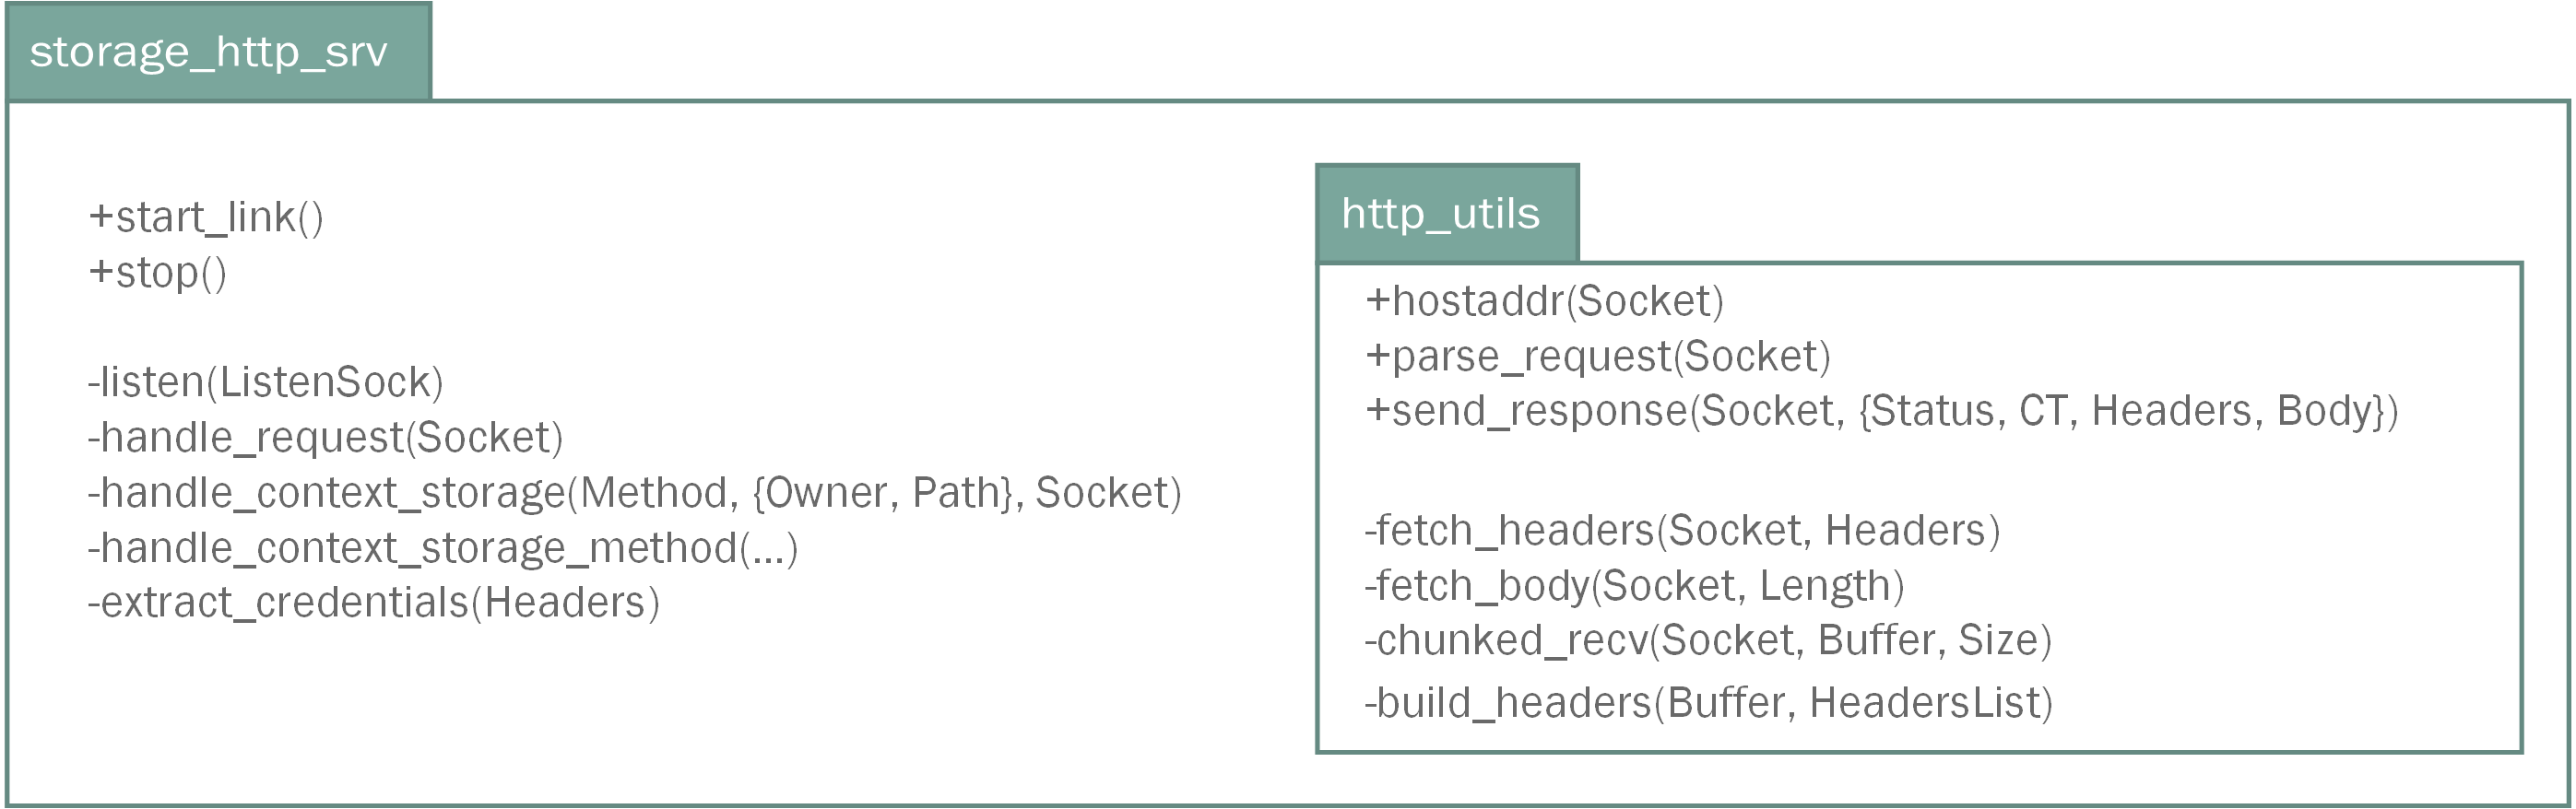
\includegraphics[width=0.9\textwidth]{http-module}
	\caption{Struktura modułu HTTP.}
	\label{fig:http-module}
\end{figure}

Budowa przykładowego zapytania, jakie można wysłać do modułu (standardowy \textit{HTTP Request}):

\begin{lstlisting}
GET storage/user02/path/to/my/file.dat HTTP/1.1
Host: ds-01.storage.example.com:9001
Authorization: HMAC user01:6c51adc384572536d9c8a9dbcfbebf590942771f
\end{lstlisting}

Zostanie przetłumaczone na poniższą strukturę Request:

\begin{lstlisting}
-record(request, {
	type 		= 'read', 
	user 		= "user01"
	addr 		= {"user02", " path/to/my/file.dat},
	hmac 		= "6c51adc384572536d9c8a9dbcfbebf590942771f", 
	data 		= none, 
	opts 		= none 
}).
\end{lstlisting}

Jeżeli plik zostanie znaleziony a użytkownik będzie mógł go odczytać, serwer zwróci odpowiedź HTTP 200 OK, a w treści znajdzie się zawartość binarna pliku.

Diagram sekwencji obsługi przykładowego zapytania typu GET (odczyt pliku) przedstawia \autoref{fig:http-seq}.

\begin{figure}[!htbp]
	\centering
	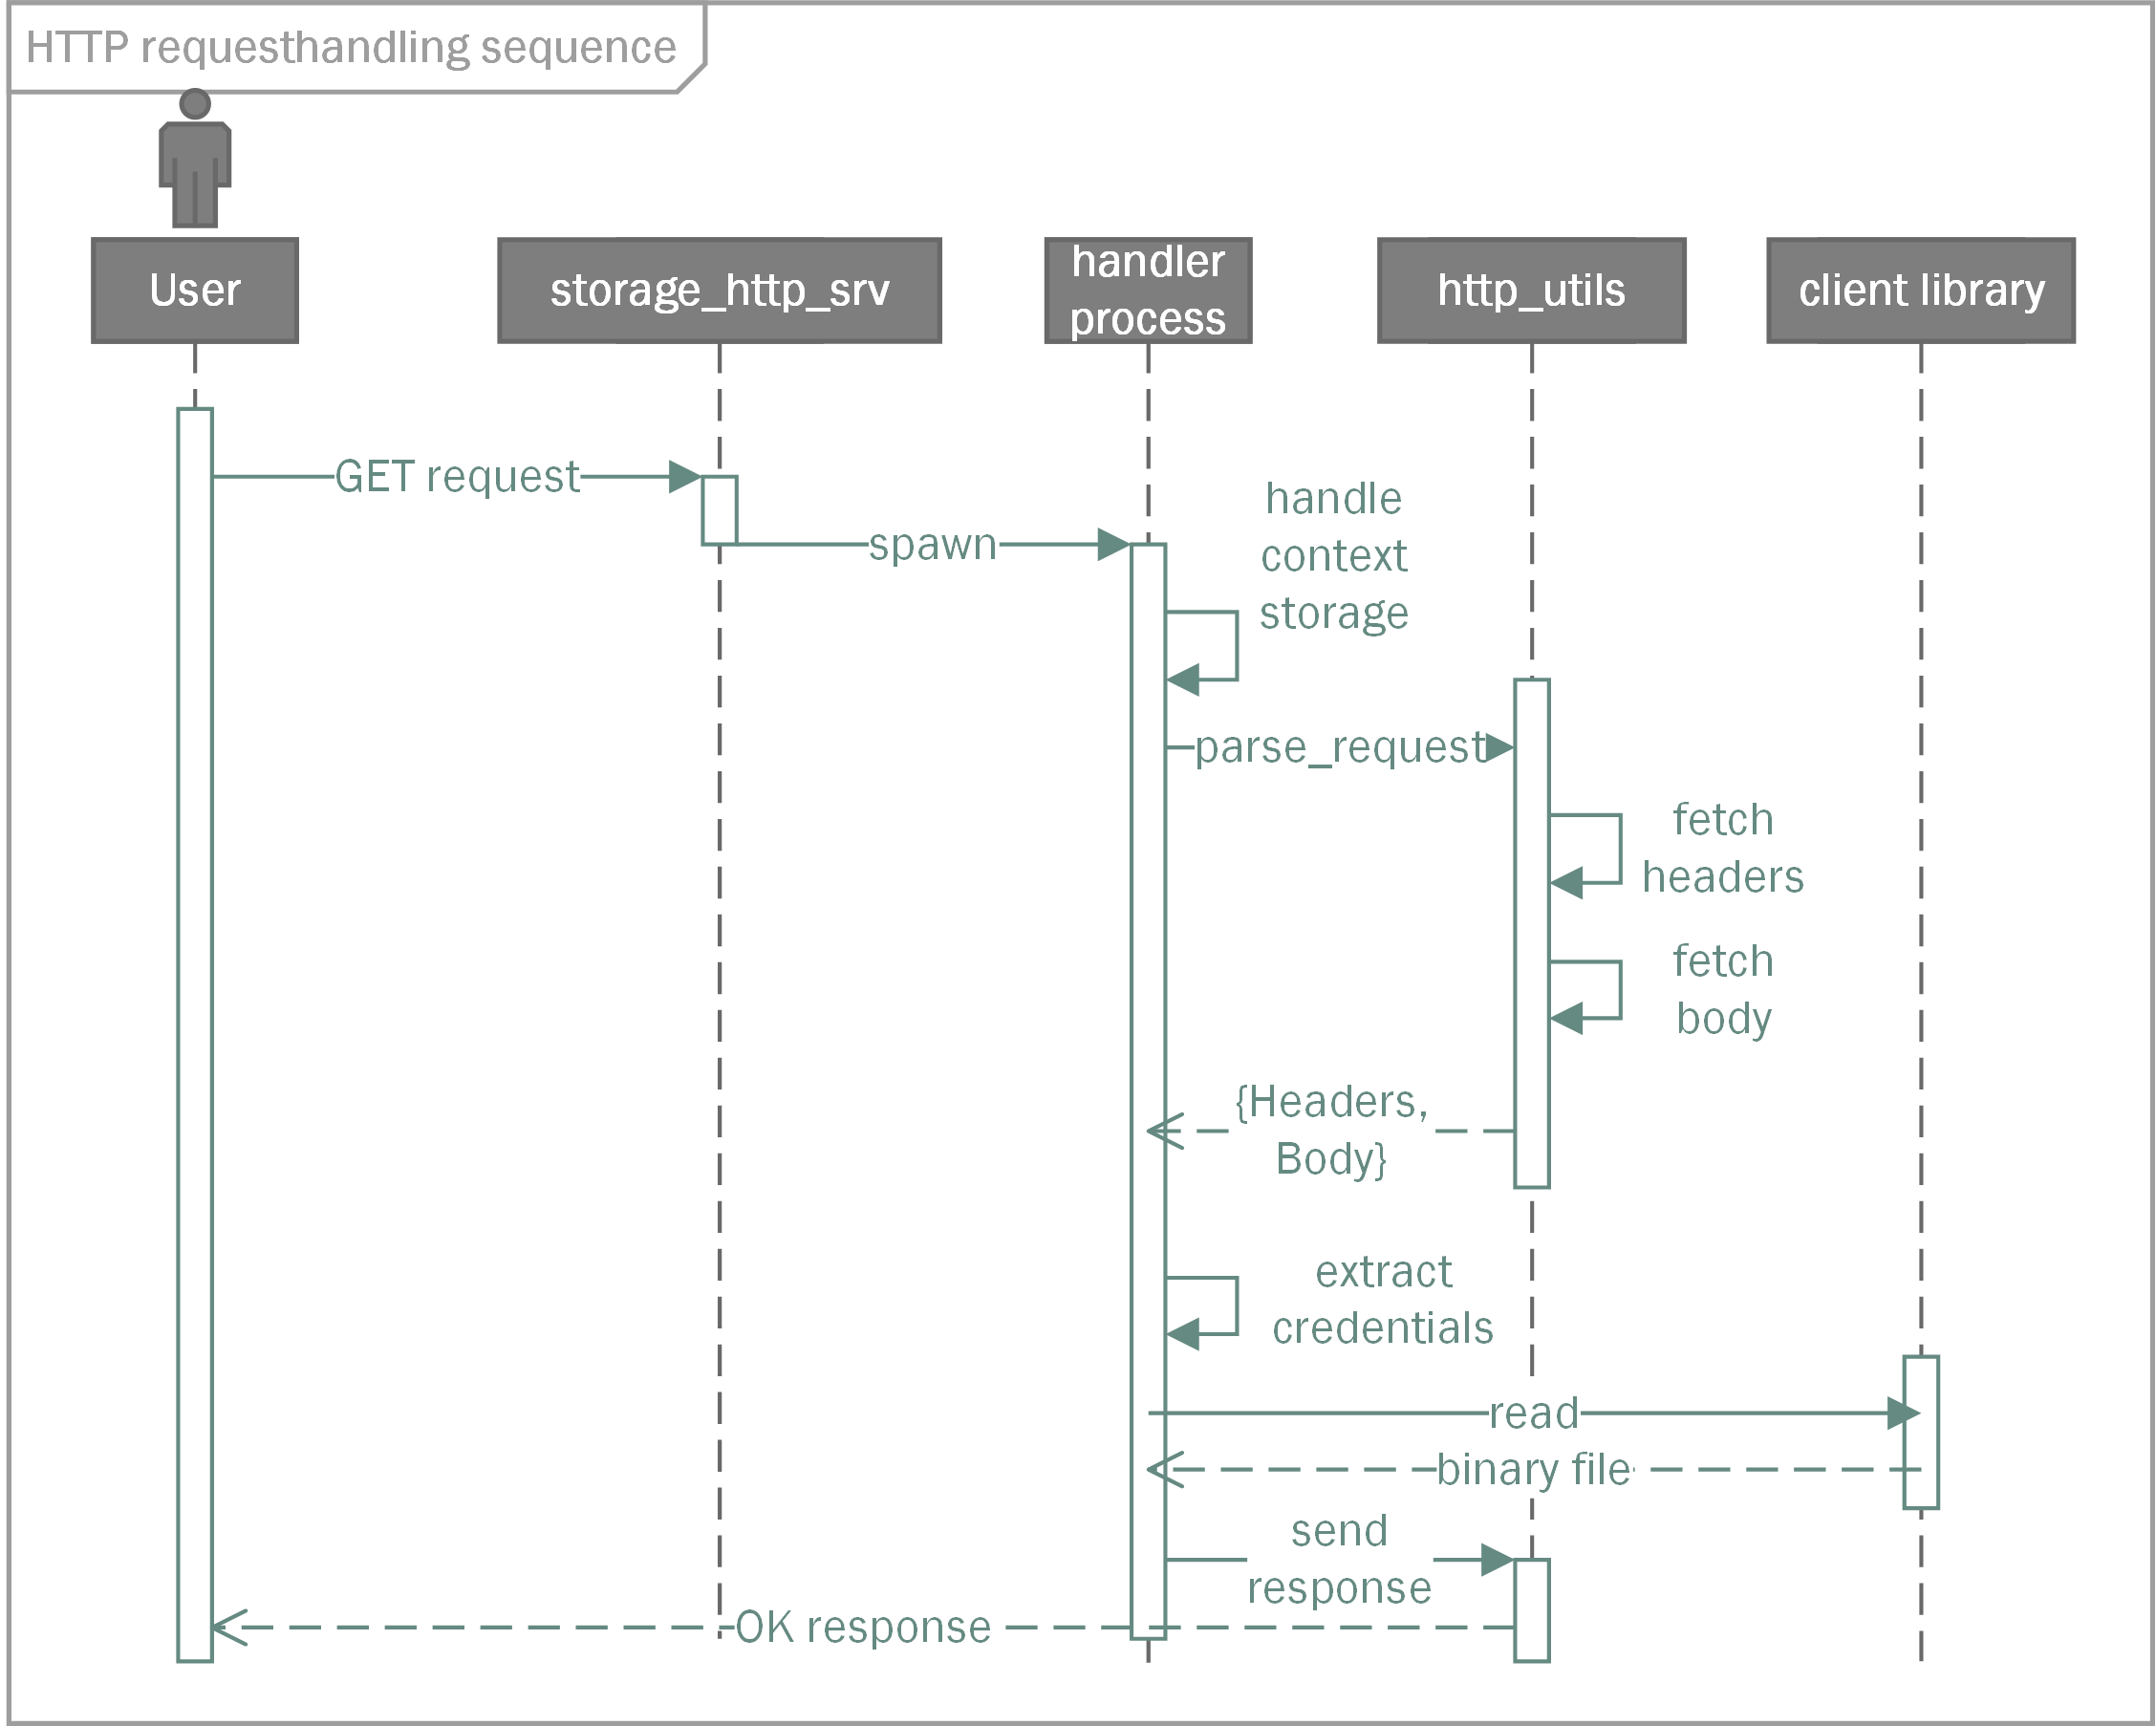
\includegraphics[width=0.9\textwidth]{http-seq}
	\caption[Przetwarzanie zapytania w module HTTP]{Przetwarzanie zapytania HTTP w module storage\_http\_srv. Dla każdego zapytania uruchamiany jest osobny wątek odpowiedzialny za jego obsługę, który parsuje zapytanie, wykonuje żądaną akcję przy użyciu biblioteki klienckiej a rezultat zwraca z powrotem przy użyciu protokołu HTTP.}
	\label{fig:http-seq}
\end{figure}